\chapter{Anforderungsanalyse}

\section{Use Case}
Die Zielgruppe dieses Projekts lässt sich relativ schwer eingrenzen. Es betrifft vor allem Personen mit Interesse in Raumfahrt oder dem Weltraum allgemein. Wichtig ist, das diese Personen keinen Bezug zur Informatik aufweisen müssen und zum Beispiel die Bedienung des User Interface daher kein Spezialwissen erfordern darf. Auch die Visualisierung der Oberfläche muss ohne Vorkenntnisse verständlich sein und dabei trotzdem noch die eigentliche Oberfläche korrekt und realitätsnah repräsentieren. Eine weitere mögliche Zielgruppe sind Schüler und Studenten, welche die Visualisierung unter anderem für Forschungszwecke nutzen können. Das Jet Propulsion Laboratory (JPL), einem Institut der NASA, welches sich auf die Entwicklung von Raumsonden und Satelliten spezialisiert, nutzt intern eine Visualisierung namens Mars Trek (siehe \ref{marsTrek}) bereits um Landeziele für Marsmissionen zu finden und plant dies auch für die Auswahl zukünftiger bemannter Erkundungsmissionen zu nutzen\ref{marsTrekLoading}. Des Weiteren könnte eine Visualisierung in den Forschungsbereichen Geologie und 
% Studium und Forschung, JPL schreibt, sie nutzen das intern um Landeziele für MArsmissionen zu finden und soll für die Auswahl zukünftiger bemannter Erkundungsmissionen genutzt werden
% Lehrende können sie nutzen, um Interesse bei Schülern im Bereich ? (Kosmologie) zu wecken oder um Kenntnisse im Bereich Geologie und Ökologie (Kunde über Natur/Vegetation) zu vermitteln

\section{Ist-Zustand}\label{istZustand}
Bevor Anforderungen definiert werden können, müssen alternative Visualisierungen in Betracht gezogen werden. Dieses Projekt soll sich dabei an gängigen Visualisierungen orientieren und versuchen deren Schwächen zu vermindern. Eine bekannte Visualisierung des JPL nennt sich Mars Trek\footnote{https://trek.nasa.gov/mars/index.html} und wurde im Jahr 2015 veröffentlicht. Es ist ein web-basiertes Tool um verschiedene Daten, gesammelt aus unterschiedlichen NASA Missionen, in einer interaktiven 3D Visualisierung zu visualisieren. Eine weitere Visualisierung versteckt sich in der Desktop Version von Google Earth [TODO]. Im folgenden werden die Alternativen beschrieben und deren Stärken und Schwächen hervorgehoben.

\subsection{Mars Trek}\label{marsTrek}
Das erste, was bei der Anwendung negativ auffällt, sind die langen Ladezeiten, die noch vor der eigentlichen Visualisierung zu sehen sind. Diese liegen beim ersten Laden der Seite im zweistelligen Sekundenbereich bis zur Sichtbarkeit der Visualisierung und ungefähr doppelt so lang bis zum vollständigen Laden der Seite (siehe \ref{marsTrekLoading} für ein durchschnittliches Laden). Nachfolgende Ladezyklen sind dann dank Cachings deutlich schneller, die Ladezeiten sind aber für ein anfangs sehr gering aufgelöstes 2D Bild trotzdem sehr hoch. Zwar sind dadurch anfangs keine visuellen Artefakte zu sehen, diese werden dann beim Bewegen der Kamera jedoch sichtbar, sodass die Nützlichkeit in Frage gestellt werden kann.

\begin{figure}[H]
  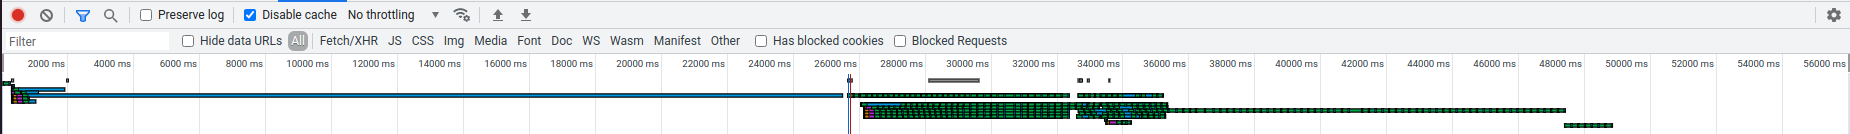
\includegraphics[width=\textwidth,keepaspectratio]{marsTrekLoading.png}
  \caption{Ladezeiten der Mars Trek Anwendung bei 50 Mbit/s auf Mittelklasse-PC}
  \label{marsTrekLoading}
\end{figure}


Initial wird man von der Anwendung mit einer 2D Ansicht des Mars mit Daten der Viking Missionen begrüßt (siehe \ref{marsTrekStart}). Zusätzlich wird dem Nutzer ein Tutorial angeboten, was auf eine relativ komplexe Anwendung schließen lässt. Die Anwendung sieht auf den ersten Blick allerdings sehr übersichtlich aus und die einzelnen Menüs lenken nicht von der eigentlichen Visualisierung ab.

\begin{figure}[H]
  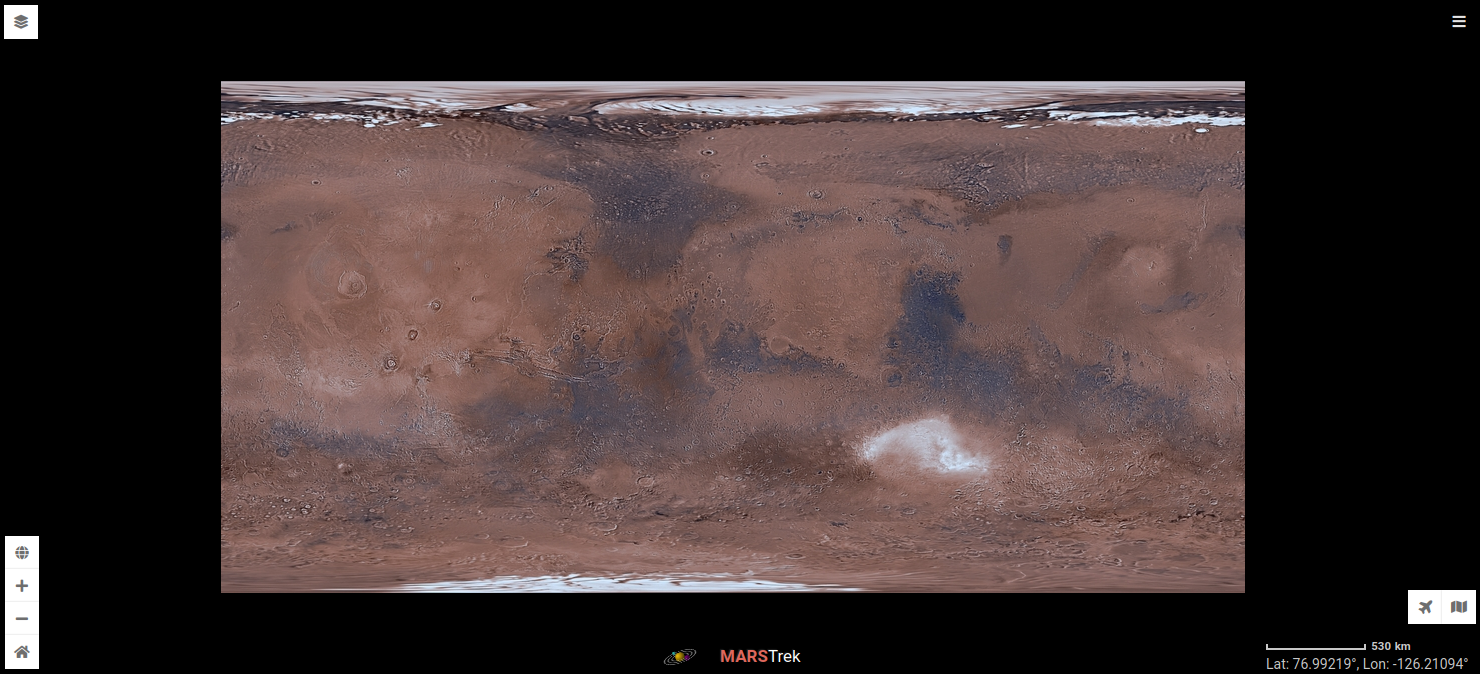
\includegraphics[width=\textwidth,keepaspectratio]{marsTrekStart.png}
  \caption{Initiale Ansicht der Mars Trek Anwendung}
  \label{marsTrekStart}
\end{figure}

Dabei befindet sich in der oberen linken Ecke ein Menü, mit dem man die verwendeten Daten auswählen kann. Unter anderem können auch MOLA Daten gewählt werden, bei denen die Höhenwerte als Farbwerte kodiert sind, ein Punkt, der auch mit diesem Projekt genutzt werden soll. Negativ fällt hier auf, dass die UI hier sehr überladen ist. Es stehen über 2000 verschiedene Datensätze zur Auswahl und die Filter nach Mission, Messinstrument, Koordinaten oder nach verschiedenen (Sub-)Kategorien ist für den Laien schwer verständlich. Auch sind nicht alle Daten für alle Flächen verfügbar, sodass teilweise nicht das gewünschte Resultat zustande kommt und sich verschiedene Ebenen nicht vollständig überlappen. Hier ist zwar ein Zeichentool vorhanden, mit dem man Ausschnitte auf der Karte definieren kann, die als weiterer Filter genutzt werden können, dies ist aber auch nicht intuitiv verständlich. 

In der unteren linken Ecke befindet sich ein Menü, mit dem man unter anderem die Projektion wechseln kann. Hier stehen eine Projektion der beiden Pole, eine globale 2D Ansicht und eine Projektion als Kugel zur Auswahl. Hier könnte das Wechseln noch intuitiver gemacht werden, da die Ansicht als 3D Modell das Highlight der Anwendung sein sollte und die derzeitige Lösung sehr versteckt ist. Des Weiteren lässt sich in dem Menü der Zoom in kleinen Schritten vergrößern und verkleinern, was durch ein Scrollen des Mausrads deutlich leichter fällt.



Alles in allem ist die Anwendung ein sehr gutes Beispiel und das generelle Design und viele Features können übernommen werden. Allerdings soll gerade im Hinblick auf eine breitere Zielgruppe die Komplexität verringert werden, indem einige Features bewusst nicht übernommen werden.



% Vergleiche die Steuerung ("standard gaming controls", man kann ja auch zwischen verschiedenen Modis umherschalten
% sie nutzen lat long in der Ecke (+ man kann zu bestimmten Koordinaten springen), haben sie auch Höheninformationen?
% ist das User Interface vielleicht überladen?

\section{Anforderungen}
Auf Grund des Prototypen-Charakters dieses Projekts besteht eine geringere Priorisierung bei den funktionalen und nicht-funktionalen Anforderungen. Es sollen möglichst viele verschiedenen Möglichkeiten zur Datenreduzierung (siehe Abschnitt \ref{datenreduzierung} implementiert und evaluiert werden. Die Anwendung soll dennoch einen Nutzen erfüllen um die Evaluation so realistisch wie möglich zu gestalten. Auch hilft dies dabei, die Korrektheit der Implementierungen zu verifizieren, wenn eine vollständige Visualisierung mit verschiedenen Features vorhanden ist. Um die konkreten Anforderungen zu ermitteln, wurden diverse Personen aus der Zielgruppe nach ihren Wünschen befragt. Aus diesen Wünschen wurden die Features priorisiert, die von den meisten Personen gewünscht wurden. Bestimmte Features, welcher im gegebenem Projektzeitraum nicht umsetzbar waren, wurden dabei im voraus verworfen. 


\subsection{Funktional}
Die wichtigste funktionale Anforderung ist eine realistische Darstellung des Mars mit den beschriebenen MOLA Daten. Dabei soll eine reine 3D Darstellung gewählt werden, 


% überlege was für Features: Farbskala muss angezeigt werden, mindestens auch der maximale und minimale Höhenwert am Rand der Skala
% Ränder der Skale sollten konfigurierbar sein, da unterschiedliche Planeten natürlich unterschiedliche Höhen aufweisen
% Ein- und Ausschalten der Projektion (Art der Projektion hängt natürlich von den verwendeten Daten ab, also sollte vom User nicht spezifiziert werden können)
% latitude, longitude und altitude für einen Punkt auf dem Globus, wie krieg ich den User dazu zu erkennen, dass er da rauf klicken muss?
% eigenes Konfigurationen für Einheiten (radians vs degrees, metrisch vs imperial) wünschenswert



\subsection{Nicht-Funktional}
Die nicht-funktionalen Anforderungen richten sich hauptsächlich an die Qualität der Visualisierung und die Performance. Hier ist es schwer, die formulierten Wünsche in konkrete Anforderungen umzuwandeln, da hier oft subjektive Dinge eine Rolle spielen. Auch lassen sich bestimmte Dinge wie die Performance einfach nicht in der gewünschten Qualität (z.B. in der Form x Frames Per Second (FPS) auf Hardware y) definieren. Insbesondere die Hardwareanforderungen können dabei auf Grund der Hardwarevielfalt nicht genau definiert werden. Eine Kernaussage ist, dass die Anwendung möglichst immer die höchste Datenauflösung anzeigt, die möglich ist. Wie bereits beschrieben (siehe Abschnitt \ref{datenmenge}) ist ein dauerhaftes Anzeigen der höchstmöglichen Datenauflösung auf normaler Hardware einfach nicht umsetzbar. Daher soll die Auflösung immer genau so hoch gewählt werden, dass eine dauerhafte Framerate von ungefähr 30 FPS erreicht wird. Die Framerate sollte möglichst genau getroffen werden, eine Abweichung darunter schadet der User Experience (UX), eine Abweichung darüber erlaubt eine Verbesserung der Datenauflösung. Hier ist also ein sehr starkes Ringen zwischen Performance und Qualität vorhanden. Der Wert wurde, anstatt der üblichen 60 FPS, nur auf ungefähr 30 FPS festgelegt, da die Visualisierung keine starken Bewegungen und somit keine flüssigen Übergange benötigt. Der Nutzer soll zwar die Kamera bewegen können, allerdings liegt der Fokus dabei immer noch auf der Visualisierung an sich.

Ein weiterer Aspekt ist, dass keine dedizierten Ladezeiten vorhanden sein sollen, in denen die Visualisierung nicht zu sehen ist. Dies wird häufig genutzt, um visuelle Ladeartefakte zu verstecken. Diese können zum Beispiel auftreten, wenn neue Abschnitte geladen werden müssen, nachdem der Benutzer die Kamerasicht verändert hat. Idealerweise soll auch auch ohne Ladezeiten der Nutzer nichts von der Trennung in Abschnitte mitbekommen und immer den Mars als Ganzes sehen. Dies kann zum Beispiel erreicht werden, in dem die Bewegung der Kamera antizipiert wird und Abschnitte, welche als nächstes geladen werden müssten, bereits vorgeladen werden.

Wichtig ist, dass die bisherigen nicht-funktionalen Anforderungen immer abhängig von der Hardware des Nutzer sind, da die Visualisierung auf Client-Seite durchgeführt wird. Es kann also kein einheitliches Performance-Konzept geben, welches für alle Nutzer geeignet ist. Zum einen können natürlich einzelne Parameter im voraus für verschiedene Performance-Klassen per Hand definiert werden. Da dafür allerdings eine umfassende Evaluation auf unterschiedlicher Hardware notwendig ist, ist der Zeitaufwand sehr groß. Eine Alternative ist es, zur Laufzeit bestimmte Parameter an die aktuellen Hardware anzupassen. Ein Problem bei beiden Ansätzen ist auch das Erfassen der aktuellen Hardware an sich. Auch ohne sich bereits auf eine Sprache oder Plattform festgelegt zu haben, gibt es meist keinen einheitlichen Weg diese zur Laufzeit zu erfassen. Natürlich könnte man den Nutzer nach der gewünschten Qualität fragen. Dieser Ansatz wird in der Realität sehr oft durchgeführt, allerdings soll die Zielgruppe kein Spezialwissen benötigen und Kenntnisse über die aktuelle Hardware sind nicht überall vorhanden. Ein Ansatz wäre es sich nicht auf die Hardware an sich zu konzentrieren, sondern zur Laufzeit die Auswirkungen zu messen und sich dementsprechend anzupassen. Man könnte zum Beispiel Parameter wie die Framerate als Indikator nutzen und dann zur Laufzeit auf Schwankungen reagieren. Alles in allem soll dieses Projekt als Prototyp dienen und ein Finetuning aller Parameter würde den Projektrahmen sprengen. Daher sind die bisher beschriebenen Anforderungen fakultativ und eher als ungefähre Richtwerte zu verstehen.

Eine Anforderung, auf die großen Wert gelegt werden soll, ist die Skalierbarkeit der Anwendung. Das Ziel dieses Projekts ist die Evaluation von verschiedenen Methoden zur Datenreduzierung. Dies soll idealerweise nicht von den verwendeten Daten abhängen und muss universell funktionieren. Die gesamte Anwendung, mit Ausnahme von Modulen die spezifische Datenformate interpretieren, muss also mit dieser Anforderung gestaltet werden. Ein Kernaspekt dieser Anforderung ist eine strikte Begrenzung von Arbeitsspeicher (RAM) und Grafikkartenspeicher (VRAM). Diese beiden Performancekriterien sind gut geeignet, die Qualität der Datenreduzierung zu beurteilen. Wichtig ist auch hier, dass der verwendete Datensatz keinen Einfluss auf die Anforderung hat, die gleichen Anforderungen müssen auch für einen Datensatz gelten, der mehrere hunderte Male größer ist. Als konkrete obere Grenze wurde Richtwerte an Mittelklasse Computer verwendet und bestehen aus 8 GB für den RAM und 4 GB für den VRAM. Eine Konsequenz, die sich aus diesen Anforderung ergibt ist, dass die Quelldaten niemals vollständig in den Arbeitsspeicher geladen werden dürfen (auch wenn es für MOLA Daten mit 2 GB ausreichen würde)
